% ---------------------------------------------------------------------------
% Section: beyond the ergodic approximation (route 1: three-temperature model)
% ---------------------------------------------------------------------------
\section{Beyond the ergodic approximation}
\label{sec:aniso}
The ergodic approximation assumes that atoms of the same energy are
distributed uniformly over the energy shell, which requires the elastic
collision rate to exceed every other rate. In the final part of the ramp this
is not the case: with $7\times10^3$ thermal atoms at $65$~nK in the $80$~Hz
trap each atom collides $5$ to $7$ times per second, while the trap depth
falls by a factor of three in the same time and evaporation removes energy
along gravity only. The redistribution of energy between the trap axes takes
about $2.7$ collisions per atom [VALUE?: Monroe et al. 1993, verify], i.e.
$0.4$ to $0.5$~s at the end of the ramp. To estimate the consequence we have
replaced the single energy distribution of the ergodic model by three thermal
energies $E_x$, $E_y$, $E_z$, one per trap axis, coupled at the rate
$\gamma_{\rm coll}/2.7$, with evaporation acting on the vertical energy only
(escape rate $c_{\rm ev}\gamma_{\rm coll}e^{-U_t/k_BT_z}$), the uniform loss
on all three, and the condensate exchanging atoms with the cloud at the rate
$2\gamma_{\rm coll}(N_{\rm th}/N_{\rm sat}-1)(N_c+1)$, where
$N_{\rm sat}=\zeta(3)k_B^3T_xT_yT_z/\hbar^3\omega_x\omega_y\omega_z$ is the
saturation number of the anisotropic cloud and the prefactor reproduces the
$50$~ms refilling time of the ergodic model. The trap axes are
$\omega_{x,y,z}=(1.2,0.7,1.2)\bar\omega$ from the final frequencies quoted in
Ref.~\cite{MelladoMunoz2020}, with $z$ vertical.

Calibrated on the data without K ($\eta_1=4.1$, $c_{\rm ev}=0.96$,
$\gamma_{\rm bg}=0.11$~s$^{-1}$; the depth exponent runs to its bound $p=6$,
i.e. the effective depth collapses at the end of the ramp, as the real trap
with gravity does, see below), this model reproduces $N$, $F$ and the mean
temperature of the no-K data with $\chi^2=125$ for 30 points against $240$
to $270$ for the ergodic model, and predicts for the data with K
$N(2\,{\rm s})=11.7\times10^3$ (measured $12.6\times10^3$) and $F=0.48$
($0.46$), and for four times the K density $F=0.20$ ($0.23$) [SIM]. Its
central prediction is the anisotropy: at $t=2$~s the vertical temperature is
$41$~nK and the horizontal ones $84$~nK with K ($43$ and $90$~nK without),
a ratio of two, which builds up after $t\simeq1.3$~s when the collision rate
drops below $30$~Hz [Fig.~\ref{fig:threeT}]. The horizontal temperatures of
the model with K, $84$ and $77$~nK for the two K densities, are close to the
measured $76$ and $78$~nK, whereas the mean temperatures, $70$ and $64$~nK,
are not; without K the measured $65$~nK lies between the model's vertical
and horizontal values. The model therefore does not by itself explain why
the measured temperature is higher with K than without (it predicts the
opposite ordering of the mean temperatures, $70$ against $74$~nK), but it
shows that at the end of the ramp the thermal cloud is far from ergodic and
that a temperature measured from one axis of a time-of-flight image can
differ from the energy temperature by a factor of order two. This moves the
question from the collision integral to the measurement: which axes the
Gaussian fit of Ref.~\cite{MelladoMunoz2020} weighs, and how the bimodal fit
distributes the Bose-enhanced peak of a nearly saturated cloud between the
"thermal" and the "condensed" components.

\begin{figure}[t]
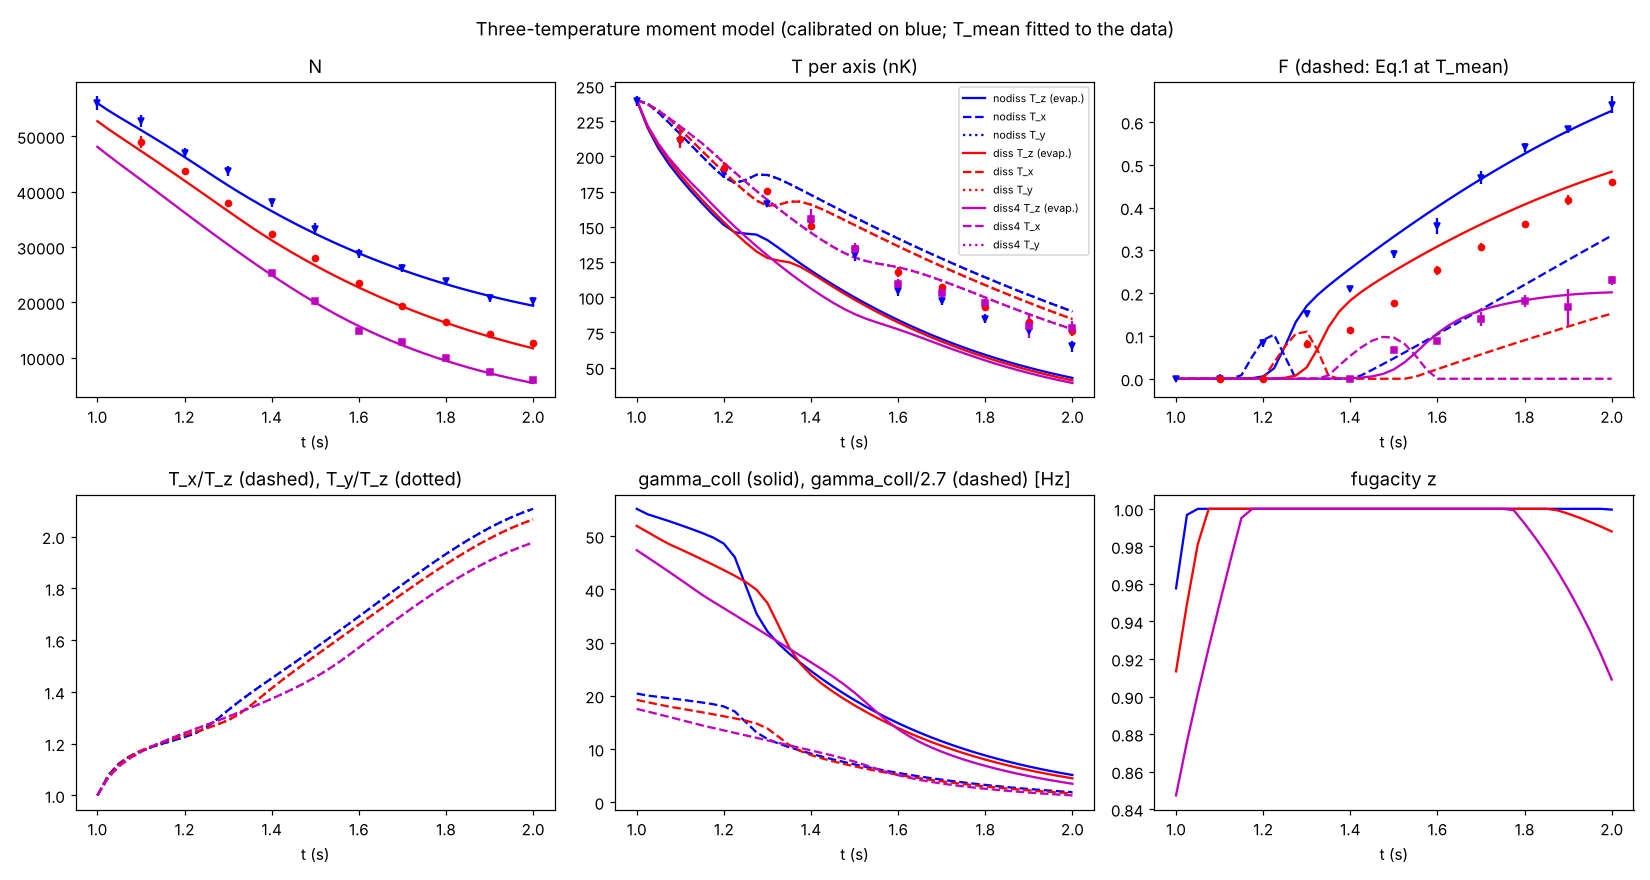
\includegraphics[width=\columnwidth]{../figures/three_temperature_ramp.png}
\caption{Three-temperature model calibrated on the no-K data (blue), with the
predictions with K (red, $\gamma_K=0.18\,t^2$~Hz) and at four times the K
density (magenta). Top: atom number, temperatures per axis (solid: vertical,
dashed and dotted: horizontal) with the measured temperatures, and condensed
fraction. Bottom: anisotropy, collision rate and its cross-axis relaxation
rate $\gamma_{\rm coll}/2.7$, and fugacity.}
\label{fig:threeT}
\end{figure}
